\documentclass[11pt, oneside]{article}   	% use "amsart" instead of "article" for AMSLaTeX format
\usepackage{geometry}                		% See geometry.pdf to learn the layout options. There are lots.
\geometry{letterpaper}                   		% ... or a4paper or a5paper or ... 
%\geometry{landscape}                		% Activate for for rotated page geometry
%\usepackage[parfill]{parskip}    		% Activate to begin paragraphs with an empty line rather than an indent
\usepackage{graphicx}				% Use pdf, png, jpg, or eps� with pdflatex; use eps in DVI mode
								% TeX will automatically convert eps --> pdf in pdflatex		
\usepackage{amssymb}
\usepackage{amsmath}
\usepackage{parskip}
\usepackage{color}
\usepackage{hyperref}

\title{Log(z)}
%\author{The Author}
%\section{}
%\subsection*{}
\date{}							% Activate to display a given date or no date

\graphicspath{{/Users/telliott_admin/Dropbox/Tex/png/}}
% \begin{center} 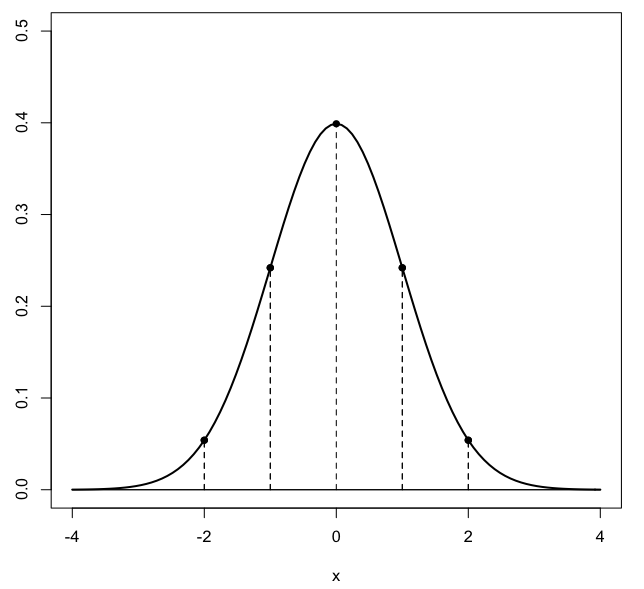
\includegraphics [scale=0.4] {gauss3.png} \end{center}
\begin{document}
\maketitle
\Large
Nearly everything works for $z$ similarly to the real numbers, except for the issue of multiple phase angles or complex arguments.  For example
\[ \log(z) = \log(re^{i\theta}) = \ln r + i \theta \]
but we may have any multiple of $2 \pi n$ added to $\theta$
\[ \log(z) = \ln r + i (\theta + 2 \pi n) \]
We call one particular range of $2 \pi$ the range for the principal value of the function.  

For example, here it is natural to make the range go from $-\pi < \theta < \pi$.  The reason is that the negative $x$-axis consists of negative real numbers, for which the natural logarithm isn't defined, and neither is the complex logarithm.  So we exclude that from the domain of the complex logarithm.  This is called a "branch cut," and we take one particular branch of this multi-valued function.

Here is a derivation.  
\[ z = x + iy = re^{i\theta} = r(\cos \theta + i \sin \theta) \]
\[ r = |z| = \sqrt{x^2 + y^2} \]

The logarithm of $z$ is $w$
\[ w = \log z \iff e^w = z \]
So what about $w$? Well, in general, it's a complex number
\[ w = s + it \]
so
\[ e^w = e^{s + it} = e^s (\cos t + i \sin t) \]
Equating the two we get
\[ r (\cos \theta + i \sin \theta) = e^s (\cos t + i \sin t) \]
Hence
\[ s = \ln r \]
\[ t = \theta \]
\[ w = \ln r + i \theta \]
\subsection*{different base}
What is 
\[ i^i = \  ? \]
So the complex logarithm of $i$ is
\[ \log i = \ln r + i \theta = \ln 1 + i \frac{\pi}{2} =  i \frac{\pi}{2} \]
 Write
\[ a^z = (e^{\log a})^z \]
\[ i^i = (e^{\log i})^i = (e^{i \pi/2})^i = e^{-\pi/2} \]
Not only is $i$ to the $ith$ power computable, it is entirely real.  It is $\approx 0.2079$.
\subsection*{derivative}
When we studied the Cauchy-Riemann equations we showed that if $f(z)$ is differentiable, then the CRE hold.  The converse theorem is also true, that if the CRE hold, then $f(z)$ is differentiable, and its derivative is
\[ f'(z) = \frac{\partial u}{\partial x} + i \frac{\partial v}{\partial x} \]

So we have that the logarithm function is
\[ \log(z) = \ln |z| + i \theta \]
Rewriting in terms of $x$ and $y$ we have that
\[ \log (x+iy) = \ln (\sqrt{x^2 + y^2}) + i \tan^{-1} (\frac{y}{x}) \]
\[ \log (x+iy) = \frac{1}{2} \ln (x^2 + y^2) + i \tan^{-1} (\frac{y}{x}) \]
So
\[ u(x,y) = \frac{1}{2} \ln (x^2 + y^2) \]
\[ u_x = \frac{1}{2} \ \frac{2x}{x^2 + y^2} = \frac{x}{x^2 + y^2} \]
\[ u_y = \frac{y}{x^2 + y^2} \]
and 
\[ v(x,y) = \tan^{-1} (\frac{y}{x}) \]
\[ v_x = \frac{1}{1 + (y/x)^2} \ y \ (-\frac{1}{x^2}) = \frac{-y}{x^2 + y^2} \]
\[ v_y = \frac{1}{1 + (y/x)^2} \ \frac{1}{x} = \frac{x}{x^2 + y^2} \]
We see that CRE are satisfied and that means that the derivative is
\[ \ [ \ \log z \ ] ' \ = u_x + i v_x \]
\[ = \frac{x}{x^2 + y^2} + i \frac{-y}{x^2 + y^2} \] 
\[ = \frac{1}{x^2 + y^2} (x - i y) \]
\[ = \frac{1}{|z|^2} \ z* \]
\[ =  \frac{1}{zz*} \ z* = \frac{1}{z} \]
The derivative of the complex logarithm is the inverse of $z$, analogous to the real case.
 
\end{document} 